\begin{section}{Metodologia}

\subsection{Modelo do Banco}
O modelo do banco foi mostrado em aula de laborat�rio pelo professor da
disciplina e segue abaixo.

\begin{figure}[!h]
    \centering
    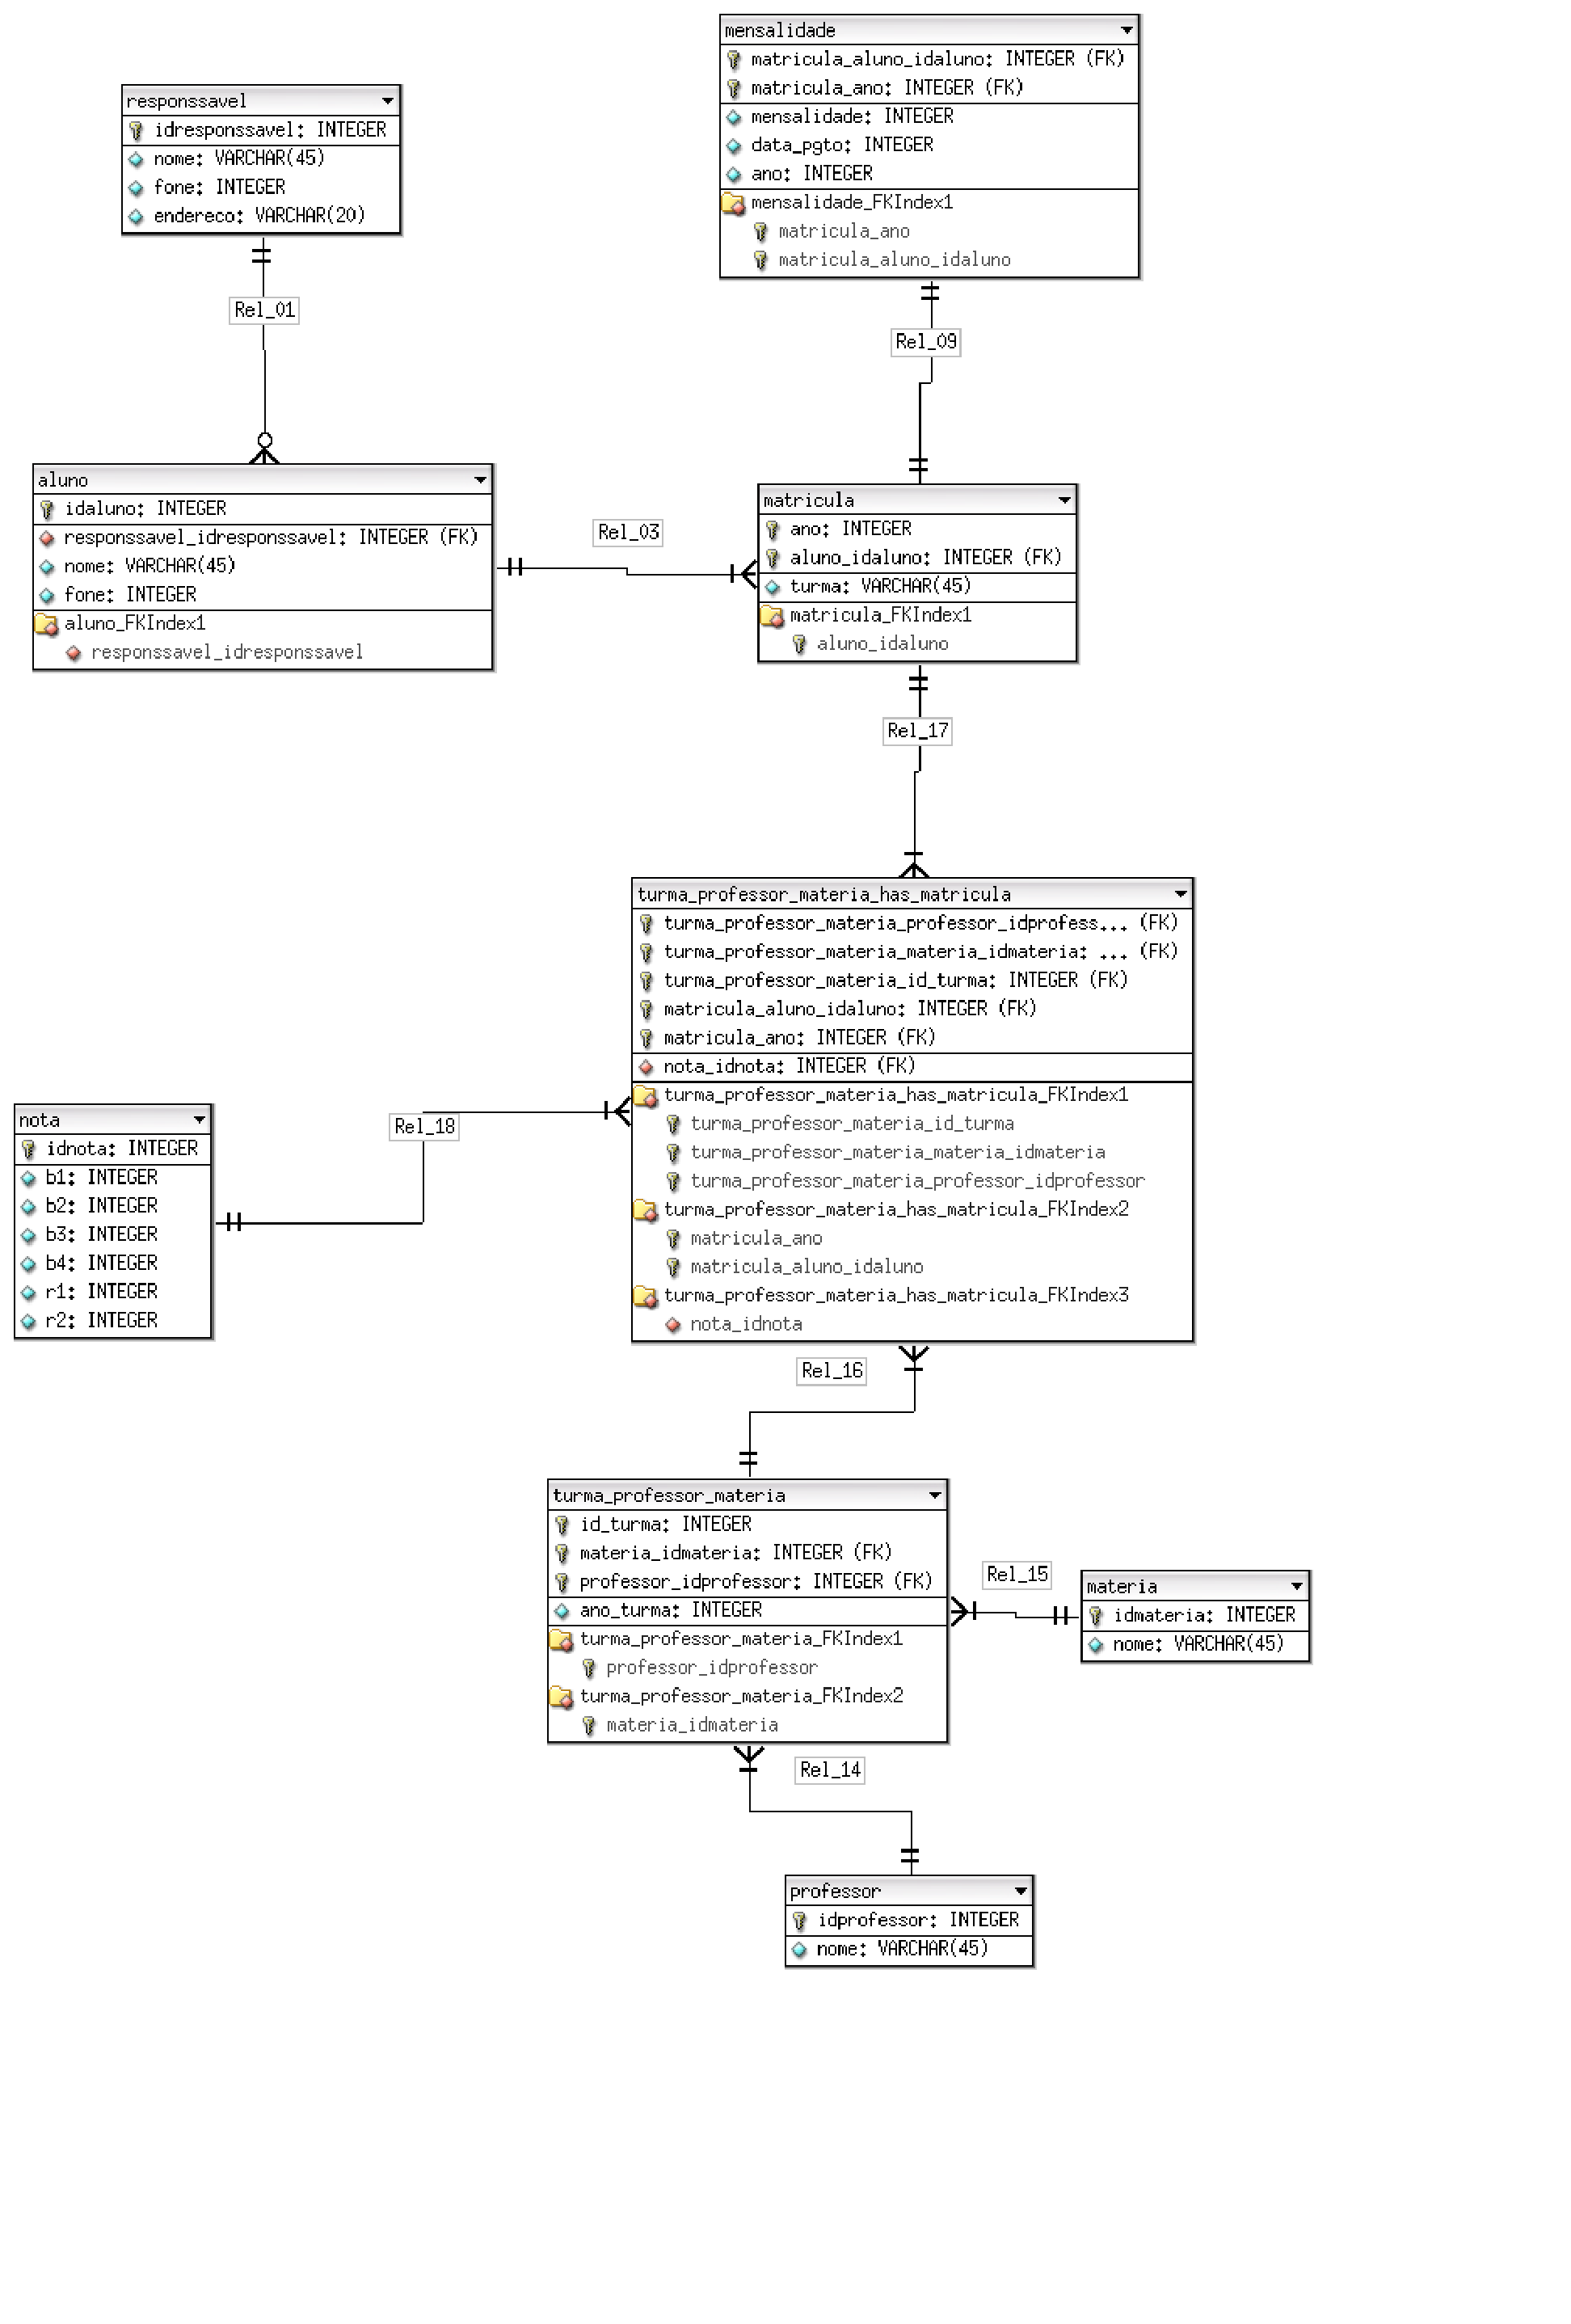
\includegraphics[width=.75\textwidth]{Figures/db_sch}
    \caption{Esquem�tio Entidade-Relacionamento}
    \label{fig:db_schema}
\end{figure}

\subsection{Cria��o do Banco}
A cria��o do Banco de dados foi feita como orientado pelo professor da
disciplina nas aulas de laborat�rio a partir do esquema \ref{fig:db_schema}feito no software
\textbf{DB Designer}.
\lstinputlisting[language=SQL]{../db_designer/db_escola_workbench_ver.sql}

\subsection{Inser��o de Valores}
A inser��o de dados no Banco foi feita como orientado no enunciado da quest�o.

\subsubsection{Respons�veis}
\lstinputlisting[language=SQL]{../db_designer/responsaveis_insertion.sql}

\subsubsection{Alunos}
\lstinputlisting[language=SQL]{../db_designer/alunos_insertion.sql}

\subsubsection{Professores}
\lstinputlisting[language=SQL]{../db_designer/professor_insertion.sql}

\subsubsection{Mat�rias}
\lstinputlisting[language=SQL]{../db_designer/materia_insert.sql}

\subsubsection{Forma��o das Turmas}
\lstinputlisting[language=SQL]{../db_designer/turma_professor_materia_insert.sql}

\subsubsection{Matr�cula}
\lstinputlisting[language=SQL]{../db_designer/Matricula_insert.sql}

subsubsection{Notas}
\lstinputlisting[language=SQL]{../db_designer/notas_insert.sql}

\subsubsection{Mensalidade}
\lstinputlisting[language=SQL]{../db_designer/mensalidade_insert.sql}

\end{section}

%%% EOF %%%
